\section{含参期望}
\label{sec:pgrad-parametric}

参数$\bm{\theta}\in\Theta\subseteq\mathbb{R}^{k}$对应一族概率分布$P_{\bm{\theta}}$和一族被积函数$f_{\bm{\theta}}$，记
\begin{equation}
  J(\bm{\theta})=\mathbb{E}_{\bm{\theta}}[f_{\bm{\theta}}(X)]=\int f_{\bm{\theta}}(x)\,P_{\bm{\theta}}(\mathrm{d}x),
  \label{eq:pgrad-J}
\end{equation}
其中$\mathbb{E}_{\bm{\theta}}$表示$X\sim P_{\bm{\theta}}$时的期望。称这样的$J$为\term{含参期望}（parameter-dependent expectation）。目标是用样本计算梯度$\nabla J(\bm{\theta})\in\mathbb{R}^{k}$。在动手构造估计之前，有两件事要先弄清：参数改变了期望里的哪些量，以及什么时候允许把求导移进期望。

\paragraph{参数进入期望的位置}

计算期望要做三件事：按某种规律产生样本，在样本处求函数值，再按概率加权平均。参数可以在其中任何一处起作用。图~\ref{fig:pgrad-three-entries}把三种位置并排画出。

\begin{BookInlineFigure}
  \centering
  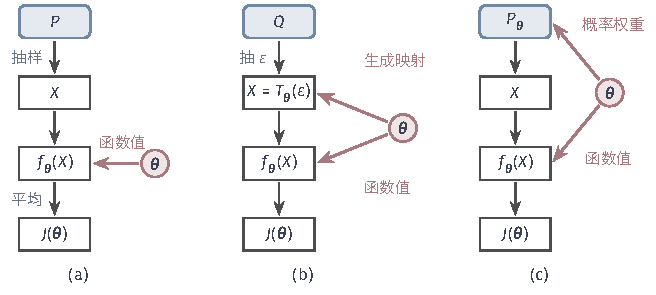
\includegraphics[width=111mm]{figures/07-probability/08-sampling-and-integration/tikz/pgrad-three-entries/figure.pdf}
  \caption{参数进入含参期望的三个位置。每列自上而下是随机性的来源、样本、函数值和期望；红色圆点标出参数进入之处。(a)抽样分布$P$固定，参数只改变函数值；(b)样本由固定分布$Q$的噪声$\varepsilon$经含参映射$T_{\bm{\theta}}$生成，参数既改变生成映射也改变函数；(c)参数改变分布$P_{\bm{\theta}}$本身，即改变各处的概率权重，同时也可以改变函数。}
  \label{fig:pgrad-three-entries}
\end{BookInlineFigure}

第一处是函数值：$f_{\bm{\theta}}(x)$在同一个$x$上随$\bm{\theta}$改变。第二处是概率权重：若$P_{\bm{\theta}}$有相对某个固定参考测度$\nu$的密度$p_{\bm{\theta}}$，参数改变的是各位置上的密度，即质量怎样分配。第三处是生成映射：样本写成$X=T_{\bm{\theta}}(\varepsilon)$，噪声$\varepsilon$的分布不变，参数改变的是同一个$\varepsilon$被送到哪里。

后两处描述的是同一件事的两种看法。对$X\sim\mathcal{N}(\theta,1)$，可以说“密度$p_{\theta}(x)=\varphi(x-\theta)$随$\theta$平移”，也可以说“$X=\theta+\varepsilon$，每个样本都向右挪了一段”。两种说法给出同一个分布族，计算梯度时只选一种，不能把分布的变化算两次。真正的要求是：在选定的表示里，凡是实际随参数变化的项都要计入，一项也不能漏。

\paragraph{两项相互抵消的例子}

取$X\sim\mathcal{N}(\theta,1)$与$f_{\theta}(x)=x^{2}-\theta x$。由$\mathbb{E}_{\theta}[X]=\theta$与$\mathbb{E}_{\theta}[X^{2}]=\theta^{2}+1$，得到
\[
  J(\theta)=\theta^{2}+1-\theta\cdot\theta=1 .
\]
$J$是常数，导数为零。现在把两种变化分开。固定分布在$\theta_{0}$，只让函数里的参数变成$t$，期望是
\[
  A(t)=\mathbb{E}_{\theta_{0}}[X^{2}-tX]=\theta_{0}^{2}+1-t\theta_{0},
\]
它在$t=\theta_{0}$处的斜率是$-\theta_{0}$。反过来固定函数为$f_{\theta_{0}}$，只让分布的参数变成$t$，期望是
\[
  B(t)=\mathbb{E}_{t}[X^{2}-\theta_{0}X]=t^{2}+1-\theta_{0}t,
\]
它在$t=\theta_{0}$处的斜率是$2\theta_{0}-\theta_{0}=\theta_{0}$。

两个斜率相加为零，正是$J'(\theta_{0})$。这就是二元函数$H(t_{1},t_{2})=\mathbb{E}_{t_{2}}[f_{t_{1}}(X)]$沿对角线$J(\theta)=H(\theta,\theta)$求导的链式法则（$H$在这里是多项式，可微性没有问题）。图~\ref{fig:pgrad-two-terms}在$\theta_{0}=1$处画出了三条曲线。只对函数求导会得到$-1$，只对分布求导会得到$+1$，两者都不是答案。

\begin{BookInlineFigure}
  \centering
  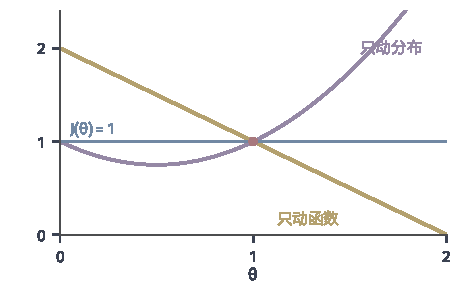
\includegraphics[width=78mm]{figures/07-probability/08-sampling-and-integration/matplotlib/pgrad-two-terms/figure.pdf}
  \caption{$X\sim\mathcal{N}(\theta,1)$，$f_{\theta}(x)=x^{2}-\theta x$。蓝线为$J(\theta)=1$；黄线为只让函数中的参数变化的$A(\theta)$；紫线为只让分布的参数变化的$B(\theta)$。三条线在红点$\theta=1$处相交，黄线斜率$-1$与紫线斜率$+1$之和等于蓝线斜率$0$。}
  \label{fig:pgrad-two-terms}
\end{BookInlineFigure}

\paragraph{期望在哪里有定义}

$J(\bm{\theta})$首先要有意义，即$f_{\bm{\theta}}$在$P_{\bm{\theta}}$下可积。例如$X\sim\operatorname{Exp}(1)$、$f_{\theta}(x)=\mathrm{e}^{\theta x}$时，
\[
  J(\theta)=\int_{0}^{\infty}\mathrm{e}^{\theta x}\mathrm{e}^{-x}\,\mathrm{d}x=\frac{1}{1-\theta},\qquad \theta<1,
\]
而$\theta\geq1$时积分发散。导数只在使$J$有定义的参数构成的开集内讨论：在某点求导，要求从该点出发朝每个方向走一小步，期望仍然有定义。因此下面总取一个以$\bm{\theta}_{0}$为中心、含在$\Theta$内的开球$U$，并检查$U$中每个参数下的可积性，而不只看$\bm{\theta}_{0}$这一点。

\paragraph{统一成固定测度上的积分}

三种参数位置可以写成同一种形式。图~\ref{fig:pgrad-three-entries}的三列分别对应
\[
  J(\bm{\theta})=\int f_{\bm{\theta}}\,\mathrm{d}P,\quad
  J(\bm{\theta})=\int f_{\bm{\theta}}(T_{\bm{\theta}}(\varepsilon))\,Q(\mathrm{d}\varepsilon),\quad
  J(\bm{\theta})=\int f_{\bm{\theta}}\,p_{\bm{\theta}}\,\mathrm{d}\nu .
\]
三个积分所对的测度$P$、$Q$、$\nu$都不随参数变化，参数全部被移进了被积函数。于是问题都化为：测度$\mu$固定，$g(\bm{\theta},x)$含参，
\begin{equation}
  J(\bm{\theta})=\int g(\bm{\theta},x)\,\mu(\mathrm{d}x)
  \label{eq:pgrad-fixed-measure}
\end{equation}
的梯度能否写成$\int\nabla_{\bm{\theta}}g(\bm{\theta},x)\,\mu(\mathrm{d}x)$。后面三节的区别只在于选哪个$\mu$和$g$，交换条件都由下面的定理检查。

\paragraph{交换的条件}

逐点可微只说明每个$x$上的函数$\bm{\theta}\mapsto g(\bm{\theta},x)$光滑，并不说明这些变化积分起来仍然受控：变化可能集中在越来越小的区域上，每个固定点都“看不到”它。需要一个与参数无关、可积的函数控制所有差商。

\begin{theorem}[积分号下求导]
\label{thm:pgrad-exchange}
设$\mu$是可测空间$\mathcal{X}$上的测度，$\bm{\theta}_{0}\in\Theta$，$U\subseteq\Theta$是以$\bm{\theta}_{0}$为中心的开球。设$g:U\times\mathcal{X}\to\mathbb{R}$满足：
\begin{enumerate}
  \item 对每个$\bm{\theta}\in U$，$g(\bm{\theta},\cdot)$可测，且$g(\bm{\theta}_{0},\cdot)$关于$\mu$可积；
  \item 对$\mu$几乎所有$x$，$\bm{\theta}\mapsto g(\bm{\theta},x)$在$\bm{\theta}_{0}$处可微；
  \item 存在$\mu$可积的函数$M\geq0$，使对$\mu$几乎所有$x$及所有$\bm{\theta},\bm{\theta}'\in U$，
  \begin{equation}
    \lvert g(\bm{\theta},x)-g(\bm{\theta}',x)\rvert\leq M(x)\lVert\bm{\theta}-\bm{\theta}'\rVert_{2}.
    \label{eq:pgrad-lipschitz}
  \end{equation}
\end{enumerate}
则对每个$\bm{\theta}\in U$，$g(\bm{\theta},\cdot)$可积，$\nabla_{\bm{\theta}}g(\bm{\theta}_{0},\cdot)$可积，式~\eqref{eq:pgrad-fixed-measure}的$J$在$\bm{\theta}_{0}$处可微，并且
\begin{equation}
  \nabla J(\bm{\theta}_{0})=\int\nabla_{\bm{\theta}}g(\bm{\theta}_{0},x)\,\mu(\mathrm{d}x).
  \label{eq:pgrad-exchange}
\end{equation}
\end{theorem}

\begin{proof}
先看可积性。由式~\eqref{eq:pgrad-lipschitz}取$\bm{\theta}'=\bm{\theta}_{0}$，对几乎所有$x$有
\[
  \lvert g(\bm{\theta},x)\rvert\leq\lvert g(\bm{\theta}_{0},x)\rvert+M(x)\lVert\bm{\theta}-\bm{\theta}_{0}\rVert_{2},
\]
右边可积，所以$g(\bm{\theta},\cdot)$可积，$J$在$U$上有定义。

再看梯度本身。记$\bm{v}(x)$为$g(\cdot,x)$在$\bm{\theta}_{0}$处的梯度，它的第$j$个分量是差商$\bigl(g(\bm{\theta}_{0}+h\bm{e}_{j},x)-g(\bm{\theta}_{0},x)\bigr)/h$沿$h=1/m\to0$的极限，是可测函数的极限，因而可测。由式~\eqref{eq:pgrad-lipschitz}，这些差商的绝对值都不超过$M(x)$，所以
\[
  \lVert\bm{v}(x)\rVert_{2}\leq\sqrt{k}\,M(x),
\]
$\bm{v}$可积。

最后证明可微。任取$\bm{h}_{m}\to\bm{0}$，$\bm{h}_{m}\neq\bm{0}$，$\bm{\theta}_{0}+\bm{h}_{m}\in U$，令
\[
  R_{m}(x)=\frac{g(\bm{\theta}_{0}+\bm{h}_{m},x)-g(\bm{\theta}_{0},x)-\langle\bm{v}(x),\bm{h}_{m}\rangle}{\lVert\bm{h}_{m}\rVert_{2}}.
\]
由条件2，对几乎所有$x$有$R_{m}(x)\to0$。由式~\eqref{eq:pgrad-lipschitz}与上一步的界，
\[
  \lvert R_{m}(x)\rvert\leq M(x)+\lVert\bm{v}(x)\rVert_{2}\leq(1+\sqrt{k})M(x).
\]
控制收敛定理给出$\int R_{m}\,\mathrm{d}\mu\to0$，也就是
\[
  \frac{J(\bm{\theta}_{0}+\bm{h}_{m})-J(\bm{\theta}_{0})-\bigl\langle\int\bm{v}\,\mathrm{d}\mu,\bm{h}_{m}\bigr\rangle}{\lVert\bm{h}_{m}\rVert_{2}}\to0 .
\]
序列$\bm{h}_{m}$是任取的，这正是$J$在$\bm{\theta}_{0}$处可微且梯度为$\int\bm{v}\,\mathrm{d}\mu$的定义。
\end{proof}

控制收敛定理的条件与证明可参考\BookChapterRef{chap:integration}{卷四第6章“积分”}。三个条件各管一件事。开球保证可以朝任意方向走一小步，并且沿线段比较。条件2只要求在$\bm{\theta}_{0}$这一点可微，例如$g(\theta,x)=\lvert\theta+x\rvert$在$\theta+x=0$处不可微，但对固定的$\theta_{0}$，这样的$x$只有一个，只要$\mu$在这一点没有质量，就不影响结论。条件3是关键：常数$M(x)$不能依赖参数，而且要对$x$可积。

常用的充分条件是梯度的一致控制。若对几乎所有$x$，$g(\cdot,x)$在整个$U$上可微，并且
\[
  \sup_{\bm{\theta}\in U}\lVert\nabla_{\bm{\theta}}g(\bm{\theta},x)\rVert_{2}\leq M(x),
\]
则沿连接$\bm{\theta}'$与$\bm{\theta}$的线段用中值定理，即得式~\eqref{eq:pgrad-lipschitz}。高斯族里的多项式函数就适合这样检查：参数限制在有界球内时，梯度不超过某个多项式乘以$\mathrm{e}^{-cx^{2}}$，后者可积。

\paragraph{逐点可微而交换失败}

下面的例子说明条件3不能省。取$U\sim\operatorname{Unif}(0,1)$，对$u\in(0,1)$令
\[
  g(\theta,u)=\frac{2\theta^{3}u}{(u^{2}+\theta^{2})^{2}},\qquad g(0,u)=0 .
\]
对每个固定的$u>0$，$g(\cdot,u)$是$\theta$的光滑函数。在$\theta=0$处，差商
\[
  \frac{g(\theta,u)-g(0,u)}{\theta}=\frac{2\theta^{2}u}{(u^{2}+\theta^{2})^{2}}\to0\qquad(\theta\to0),
\]
所以逐点导数为零，积分后仍是零。

另一方面，令$w=u^{2}+\theta^{2}$，$\mathrm{d}w=2u\,\mathrm{d}u$，对$\theta\neq0$有
\[
  J(\theta)=\theta^{3}\int_{\theta^{2}}^{1+\theta^{2}}w^{-2}\,\mathrm{d}w=\theta^{3}\Bigl(\frac{1}{\theta^{2}}-\frac{1}{1+\theta^{2}}\Bigr)=\frac{\theta}{1+\theta^{2}} .
\]
这个式子在$\theta=0$也成立，于是$J'(0)=1\neq0$。

失败的原因在图~\ref{fig:pgrad-moving-spike}(a)中一目了然。$g(\theta,\cdot)$是一个高度固定（约$0.65$）、宽度与$\theta$成正比的尖峰，$\theta\to0$时它被挤向$u=0$，面积约为$\theta$。每个固定的$u$最终都落在尖峰右侧，只看到函数值趋于零；尖峰携带的面积却以斜率$1$消失。用定理的语言说：对$\theta$求偏导数，
\[
  \partial_{\theta}g(\theta,u)=\frac{2u\bigl(3\theta^{2}(u^{2}+\theta^{2})-4\theta^{4}\bigr)}{(u^{2}+\theta^{2})^{3}},
\]
在$\theta=u$处它等于$1/(2u)$。任何满足式~\eqref{eq:pgrad-lipschitz}的$M$都要在$(0,\delta)$上不小于$1/(2u)$，而$\int_{0}^{\delta}\frac{1}{2u}\,\mathrm{d}u=\infty$。被积函数本身有界、逐点光滑，仍然不够。

\begin{BookInlineFigure}
  \centering
  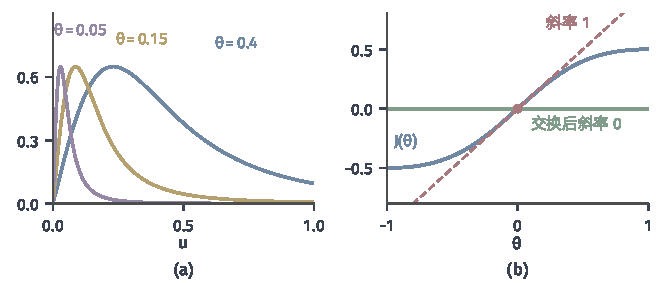
\includegraphics[width=112mm]{figures/07-probability/08-sampling-and-integration/matplotlib/pgrad-moving-spike/figure.pdf}
  \caption{逐点可微而不能交换求导与积分。(a)$g(\theta,u)=2\theta^{3}u/(u^{2}+\theta^{2})^{2}$在$\theta=0.4,0.15,0.05$时的图像，峰高都约为$0.65$，峰向$u=0$移动并变窄。(b)蓝线为$J(\theta)=\theta/(1+\theta^{2})$，红色虚线是它在原点处斜率为$1$的切线，绿线是逐点求导后再积分得到的斜率$0$。}
  \label{fig:pgrad-moving-spike}
\end{BookInlineFigure}

这个例子也说明了为什么检查要放在参数的一个邻域上，而不只在$\bm{\theta}_{0}$：在$\theta=0$这一点，每个$u$处的导数都存在且有界，毛病出在$\theta$离开零的过程中。后面每种梯度表示都先写成式~\eqref{eq:pgrad-fixed-measure}的形式，再用定理~\ref{thm:pgrad-exchange}检查。
